\section{Impossibility of an Additive $\FPTAS$}\label{sec:hardness}

In this section, we show that the additive $\PTAS$ obtained in the previous section is tight. In particular, we show that the single-dimensional Bayesian principal-agent problem does not admit an additive $\FPTAS$, even if the distribution has finite support. As it is customary for distributions with finite support, we assume that the distribution $\Gamma$ is represented by a tuple $(\gamma_\theta)_{\theta \in \supp(\Gamma)}$.

\begin{theorem}\label{thm:reduction}
The single-dimensional Bayesian principal-agent problem does not admit an additive $\FPTAS$, unless $\PolyClass=\NP$.
\end{theorem}

\paragraph{Challenges in Hardness of Single-Dimensional Contract Design}

When proving the hardness of multi-dimensional contract design, a recurrent feature that is exploited is the fact that an agent of type $\theta$ essentially has different parameters. For example, we could easily implement an instance in which the set of actions is different for each agent.\footnote{
Not all existing reductions adopt this framing. For example, in the reduction by \citet{guruganesh2021contracts}, this is achieved by assigning a distinct outcome distribution to each type $\theta$. However, this is essentially equivalent to having a different set of actions, as presented in our discussion.}
%
Next, we provide a high-level intuition on how this can be leveraged into a reduction. For example, if reducing from \textsc{Set-Cover}, one can have a type for each element of the universe $E$ and an outcome for each set $S$ in the universe $\Scal$. Then, a type corresponding to an element in the universe can only play actions that lead deterministically to a ``favorable outcome'' $\omega_S$. For any cover $\Scal^\star\subseteq\Scal$, we can thus construct a contract that incentivizes an action that leads to $\omega_S$ if $S\in\Scal^\star$. Since $\Scal^\star$ is a cover of $E$, each agent has an action that leads to a favorable outcome, and thus, the utility of the player is large. The fundamental property of this reduction is that an agent of a type corresponding to an element $i$ can only induce outcomes $\omega_S$ such that $i\in S$. However, this is not the case in single-dimensional settings.% in which all agents share the same action set, outcome distributions, and costs.
Indeed, the main technical challenge in proving hardness in the single-dimensional setting is that all agents have the same action set, outcomes, and outcome distributions. They can only differ in their costs, and only by a multiplicative factor! This constraint makes proving hardness results challenging in single-dimensional settings, as it requires artificially ``separating'' actions.



\paragraph{Previous Approach} The closest construction to ours is presented in~\citet{castiglioni2025reduction}, which reduces multi-dimensional to single-dimensional contract design, preserving \emph{multiplicative} approximations. 
%
One crucial feature of their approach is the use of sequences of exponentially decreasing costs and expected rewards.
%
Sequences of exponentially decreasing costs and expected rewards are very effective in creating ``separation'' among actions, making some actions clearly suboptimal for an agent of a given type.
%
At a high level, their approach essentially partitions the set of actions, guaranteeing that only inducing the agent to play a subset of action (the ones available to the type in the multi-dimensional instance) provides a non-negligible reward to the principal.
%
While this is effective for multiplicative approximations, it results in the principal’s expected utility becoming exponentially small as the instance size increases. In such instances, approximately optimal contracts can be efficiently found under additive approximation. Indeed, posting the null contract provides an additive error that is trivially exponentially small in the instance size.
%\mat{"exponentially small in the instance size" non capisco se è formalmente corretto}

\paragraph{High-Level Construction} For the reason above, we recognized the need to use polynomially decreasing sequences of costs and expected rewards, which require a much more fine-grained analysis to establish such separation. Here, we outline the construction of our sequences, temporarily setting aside the additional complexities of the reduction.
% Hence, we realized that we have to use polynomially decreasing sequences of costs and expected rewards, which require a much more fine-grained analysis in order to prove such separation.
% %
% Here, we provide a sketch of the construction of our sequences, in which we ignore all the additional difficulties of the reduction.
%
The goal is to find a sequence of outcome distributions $F_{a_i,\omega}$,  action costs $c_{a_i}$, and a sequence of types $\theta_i$, where $i \in \mathbb{N}$, such that, when the contract is set to $p_{\omega}=1$, then the best response of a type $\theta_i$ is $a_i$.
We construct such sequence as follows: for each $i$, we set
\begin{itemize}
\item $F_{a_i,\omega}= \frac{1}{2i} $;
\item $c_{a_i}=\frac{1}{4i^2}$;
\item  types $\theta_i=i$.
\end{itemize}
%
Then, an agent of type $i$ will play the action maximizing their utility:
\[
i=\arg \max_{j \in \mathbb{N}} \left[ p_\omega F_{a_j,\omega} -\theta_{i}c_{a_j} \right] =\arg \max_{j \in \mathbb{N}} \left[ \frac{1}{2j} -\frac{i}{4j^2} \right], 
\]
which is the action corresponding to its type, as desired.
\begin{figure}[!t]
    \centering
    \scalebox{0.7}{\tikzset{every picture/.style={line width=0.75pt}} %set default line width to 0.75pt        

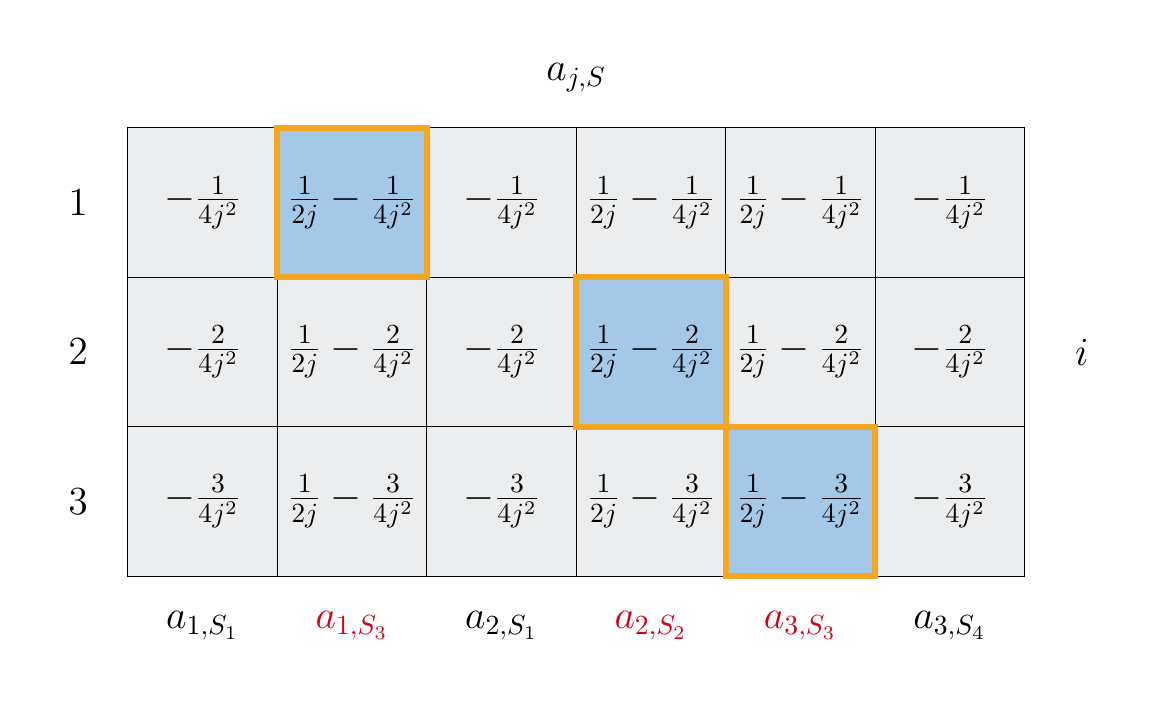
\begin{tikzpicture}[x=0.75pt,y=0.75pt,yscale=-1.2,xscale=1.2]
%uncomment if require: \path (0,447); %set diagram left start at 0, and has height of 447

\definecolor{niceRed}{RGB}{190,38,38}
\definecolor{Red2}{RGB}{219, 50, 54}
\definecolor{mgreen}{RGB}{160, 200, 140}
\definecolor{blueGrotto}{RGB}{5,157,192}
\definecolor{limeGreen}{HTML}{81B622}
\definecolor{myellow}{rgb}{0.88,0.61,0.14}
\definecolor{darkGreen}{HTML}{2E8B57}
\definecolor{navyBlueP}{HTML}{03468F}
\definecolor{Sepia}{HTML}{7F462C}
\definecolor{red2}{HTML}{1F462C}
\definecolor{orange2}{HTML}{FF8000}
\definecolor{mgray}{HTML}{ABB3B8}
\definecolor{lgray}{HTML}{E5E8E9}
\definecolor{myPurple}{RGB}{175,0,124}
\definecolor{mypurple2}{rgb}{0.8,0.62,1}
\definecolor{royalBlue}{HTML}{057DCD}
\definecolor{mpink}{HTML}{FC6C85}
\definecolor{lblue}{RGB}{74,144,226}
\definecolor{peagreen}{RGB}{152,193,39}
\definecolor{typ_navy}{HTML}{001f3f}
\definecolor{typ_blue}{HTML}{0074d9}
\definecolor{typ_aqua}{HTML}{7fdbff}
\definecolor{typ_teal}{HTML}{39cccc}
\definecolor{typ_eastern}{HTML}{239dad}
\definecolor{typ_purple}{HTML}{b10dc9}
\definecolor{typ_fuchsia}{HTML}{f012be}
\definecolor{typ_maroon}{HTML}{85144b}
\definecolor{typ_red}{HTML}{ff4136}
\definecolor{typ_orange}{HTML}{ff851b}
\definecolor{typ_yellow}{HTML}{ffdc00}
\definecolor{typ_olive}{HTML}{3d9970}
\definecolor{typ_green}{HTML}{2ecc40}
\definecolor{typ_lime}{HTML}{01ff70}
\definecolor{newgreen}{HTML}{83c702}
\definecolor{newpurp}{RGB}{97,96,121}
\colorlet{highcell}{typ_blue}
\colorlet{cell}{mgray!80!}

%Shape: Square [id:dp18447254434518756] 
\draw  [fill=cell  ,fill opacity=0.3 ] (130,80) -- (190,80) -- (190,140) -- (130,140) -- cycle ;
%Shape: Square [id:dp05839107951692313] 
\draw  [fill=cell  ,fill opacity=0.3 ] (190,80) -- (250,80) -- (250,140) -- (190,140) -- cycle ;
%Shape: Square [id:dp8258865911782285] 
\draw  [fill=cell  ,fill opacity=0.3 ] (250,80) -- (310,80) -- (310,140) -- (250,140) -- cycle ;
%Shape: Square [id:dp7470787833959325] 
\draw  [fill=cell  ,fill opacity=0.3 ] (310,80) -- (370,80) -- (370,140) -- (310,140) -- cycle ;
%Shape: Square [id:dp753495709362549] 
\draw  [fill=cell  ,fill opacity=0.3 ] (370,80) -- (430,80) -- (430,140) -- (370,140) -- cycle ;
%Shape: Square [id:dp9549002339125607] 
\draw  [fill=cell  ,fill opacity=0.3 ] (430,80) -- (490,80) -- (490,140) -- (430,140) -- cycle ;
%Shape: Square [id:dp341646963367104] 
\draw  [fill=cell  ,fill opacity=0.3 ] (130,140) -- (190,140) -- (190,200) -- (130,200) -- cycle ;
%Shape: Square [id:dp7737964462419404] 
\draw  [fill=cell  ,fill opacity=0.3 ] (190,140) -- (250,140) -- (250,200) -- (190,200) -- cycle ;
%Shape: Square [id:dp24658318527861756] 
\draw  [fill=cell  ,fill opacity=0.3 ] (250,140) -- (310,140) -- (310,200) -- (250,200) -- cycle ;
%Shape: Square [id:dp8071145078445718] 
\draw  [fill=cell  ,fill opacity=0.3 ] (310,140) -- (370,140) -- (370,200) -- (310,200) -- cycle ;
%Shape: Square [id:dp29047936857326784] 
\draw  [fill=cell  ,fill opacity=0.3 ] (370,140) -- (430,140) -- (430,200) -- (370,200) -- cycle ;
%Shape: Square [id:dp4676132783562479] 
\draw  [fill=cell  ,fill opacity=0.3 ] (430,140) -- (490,140) -- (490,200) -- (430,200) -- cycle ;
%Shape: Square [id:dp1733325055006072] 
\draw  [fill=cell  ,fill opacity=0.3 ] (130,200) -- (190,200) -- (190,260) -- (130,260) -- cycle ;
%Shape: Square [id:dp013191480917102538] 
\draw  [fill=cell  ,fill opacity=0.3 ] (190,200) -- (250,200) -- (250,260) -- (190,260) -- cycle ;
%Shape: Square [id:dp862900728287235] 
\draw  [fill=cell  ,fill opacity=0.3 ] (250,200) -- (310,200) -- (310,260) -- (250,260) -- cycle ;
%Shape: Square [id:dp2923844556177173] 
\draw  [fill=cell  ,fill opacity=0.3 ] (310,200) -- (370,200) -- (370,260) -- (310,260) -- cycle ;
%Shape: Square [id:dp9262580252867507] 
\draw  [fill=cell  ,fill opacity=0.3 ] (370,200) -- (430,200) -- (430,260) -- (370,260) -- cycle ;
%Shape: Square [id:dp9940510214018494] 
\draw  [fill=cell  ,fill opacity=0.3 ] (430,200) -- (490,200) -- (490,260) -- (430,260) -- cycle ;
%Shape: Rectangle [id:dp3826764540345684] 
\draw  [draw opacity=0] (130,40) -- (490,40) -- (490,80) -- (130,80) -- cycle ;
%Shape: Rectangle [id:dp44718946645668556] 
\draw  [draw opacity=0] (490,80) -- (530,80) -- (530,260) -- (490,260) -- cycle ;
%Shape: Square [id:dp19417810783211653] 
\draw  [color={rgb, 255:red, 245; green, 166; blue, 35 }  ,draw opacity=1 ][fill=highcell  ,fill opacity=0.3 ][line width=2.25]  (190,80) -- (250,80) -- (250,140) -- (190,140) -- cycle ;
%Shape: Square [id:dp47463876768857904] 
\draw  [color={rgb, 255:red, 245; green, 166; blue, 35 }  ,draw opacity=1 ][fill=highcell  ,fill opacity=0.3 ][line width=2.25]  (310,140) -- (370,140) -- (370,200) -- (310,200) -- cycle ;
%Shape: Square [id:dp7561737741024661] 
\draw  [color={rgb, 255:red, 245; green, 166; blue, 35 }  ,draw opacity=1 ][fill=highcell  ,fill opacity=0.3 ][line width=2.25]  (370,200) -- (430,200) -- (430,260) -- (370,260) -- cycle ;
%Shape: Rectangle [id:dp1521259735983933] 
\draw  [draw opacity=0] (130,260) -- (190,260) -- (190,300) -- (130,300) -- cycle ;
%Shape: Rectangle [id:dp5821114045562574] 
\draw  [draw opacity=0] (190,260) -- (250,260) -- (250,300) -- (190,300) -- cycle ;
%Shape: Rectangle [id:dp4942755713419844] 
\draw  [draw opacity=0] (250,260) -- (310,260) -- (310,300) -- (250,300) -- cycle ;
%Shape: Rectangle [id:dp39061313661505737] 
\draw  [draw opacity=0] (310,260) -- (370,260) -- (370,300) -- (310,300) -- cycle ;
%Shape: Rectangle [id:dp783768540426248] 
\draw  [draw opacity=0] (370,260) -- (430,260) -- (430,300) -- (370,300) -- cycle ;
%Shape: Rectangle [id:dp4550864548144524] 
\draw  [draw opacity=0] (430,260) -- (490,260) -- (490,300) -- (430,300) -- cycle ;
%Shape: Rectangle [id:dp04094720606885227] 
\draw  [draw opacity=0] (90,80) -- (130,80) -- (130,140) -- (90,140) -- cycle ;
%Shape: Rectangle [id:dp43944766721634676] 
\draw  [draw opacity=0] (90,140) -- (130,140) -- (130,200) -- (90,200) -- cycle ;
%Shape: Rectangle [id:dp3966404607216445] 
\draw  [draw opacity=0] (90,200) -- (130,200) -- (130,260) -- (90,260) -- cycle ;

% Text Node
\draw (160,280) node  [font=\Large]  {$a_{1,S_{1}}$};
% Text Node
\draw (220,280) node  [font=\Large,color={rgb, 255:red, 208; green, 2; blue, 27 }  ,opacity=1 ]  {$a_{1,S_{3}}$};
% Text Node
\draw (280,280) node  [font=\Large]  {$a_{2,S_{1}}$};
% Text Node
\draw (340,280) node  [font=\Large,color={rgb, 255:red, 208; green, 2; blue, 27 }  ,opacity=1 ]  {$a_{2,S_{2}}$};
% Text Node
\draw (400,280) node  [font=\Large,color={rgb, 255:red, 208; green, 2; blue, 27 }  ,opacity=1 ]  {$a_{3,S_{3}}$};
% Text Node
\draw (460,280) node  [font=\Large]  {$a_{3,S_{4}}$};
% Text Node
\draw (310,60) node   [font=\Large] {$a_{j,S}$};
% Text Node
\draw (513,170) node  [font=\Large]  {$i$};
% Text Node
\draw (220,170) node  [font=\Large]  {$\frac{1}{2j} -\frac{2}{4j^{2}}$};
% Text Node
\draw (160,170) node  [font=\Large]  {$-\frac{2}{4j^{2}}$};
% Text Node
\draw (400,170) node  [font=\Large]  {$\frac{1}{2j} -\frac{2}{4j^{2}}$};
% Text Node
\draw (460,170) node  [font=\Large]  {$-\frac{2}{4j^{2}}$};
% Text Node
\draw (280,170) node  [font=\Large]  {$-\frac{2}{4j^{2}}$};
% Text Node
\draw (340,170) node  [font=\Large]  {$\frac{1}{2j} -\frac{2}{4j^{2}}$};
% Text Node
\draw (110,110) node  [font=\Large] {$1$};
% Text Node
\draw (110,170) node  [font=\Large] {$2$};
% Text Node
\draw (110,230) node  [font=\Large] {$3$};
% Text Node
\draw (460,110) node  [font=\Large]  {$-\frac{1}{4j^{2}}$};
% Text Node
\draw (460,230) node  [font=\Large]  {$-\frac{3}{4j^{2}}$};
% Text Node
\draw (400,230) node  [font=\Large]  {$\frac{1}{2j} -\frac{3}{4j^{2}}$};
% Text Node
\draw (400,110) node  [font=\Large]  {$\frac{1}{2j} -\frac{1}{4j^{2}}$};
% Text Node
\draw (280,230) node  [font=\Large]  {$-\frac{3}{4j^{2}}$};
% Text Node
\draw (160,230) node  [font=\Large]  {$-\frac{3}{4j^{2}}$};
% Text Node
\draw (220,230) node  [font=\Large]  {$\frac{1}{2j} -\frac{3}{4j^{2}}$};
% Text Node
\draw (340,110) node  [font=\Large]  {$\frac{1}{2j} -\frac{1}{4j^{2}}$};
% Text Node
\draw (220,110) node  [font=\Large]  {$\frac{1}{2j} -\frac{1}{4j^{2}}$};
% Text Node
\draw (280,110) node  [font=\Large]  {$-\frac{1}{4j^{2}}$};
% Text Node
\draw (160,110) node  [font=\Large]  {$-\frac{1}{4j^{2}}$};
% Text Node
\draw (340,230) node  [font=\Large]  {$\frac{1}{2j} -\frac{3}{4j^{2}}$};


\end{tikzpicture}}
    \caption{Stylized instance corresponding to the \textsc{Set-Cover} instance: $S_1=\{1,2\},S_3=\{2\},S_3=\{1,3\},S_4=\{3\}$ with universe $E=\{1,2,3\}$. An example of a cover is $\Scal^\star=\{S_2,S_3\}$. The table corresponds to payments $p_{\omega_{S_2}}=p_{\omega_{S_3}}=1$ while all the others are $0$. In each cell, there is the utility of an agent of type $i$ (indexed by rows) of playing an action of type $a_{j,S}$ (indexed by columns). We highlighted in \textcolor{niceRed}{red} the actions corresponding to the outcomes $\omega_{S_2}$ and $\omega_{S_3}$, and in \textcolor{typ_blue}{blue} the action played by each agent.}
    \label{fig:instance}
\end{figure}
This sequence is used when reducing from \textsc{Set-Cover} by replicating this sequence for each $S\in\Scal$ if $i\in S$. Formally, we have actions $a_{i,S}$ for each $i\in S$ and $S\in\Scal$, and outcome $\omega_S$ for each $S\in\Scal$. Then, $F_{a_{i,S},\omega_{S}}=\frac{1}{2i}$ and $c_{a_{i,S},\omega_S}=\frac{1}{4i^2}$ as above. The properties of the sequence guarantee that an agent $i$ plays an action $a_{i,S}$ for some $S\in\Scal$ if the principal picked payment $p_{\omega_S}=1$. Thus for a cover $\Scal^\star$ we can choose payments $p_{\omega_S}=\mathbb{I}(S\in\Scal^\star)$, and each agent of type $i$ has an action $a_{i,S}$ to play.
%
%
\Cref{fig:instance} provides depiction of the sequence associated with a simple \textsc{Set-Cover} instance. 
In the next section, we provide the formal proof of \Cref{thm:reduction}.

\subsection{Proof of \Cref{thm:reduction}}

	We reduce from \textsc{Set-Cover}.
	%
	Given a set of elements $E$ and a set of sets $\Scal \subseteq 2^E$, we reduce from the decision problem of determining if there exists a set cover of size $k$, i.e., a set $\Scal^\star\subseteq \Scal$ of size $k$ such that 
	$\bigcup_{S \in \Scal^\star} S=E$. This problem is well known to be NP-Hard \cite{Karp1972}.
	
	We show that if there exists a set cover of size $k$, then principal's utility from the optimal contract is at least $\ell$ where $\ell$ will be defined in the following, while if all the set covers have size at least $k+1$ then the utility is at most $\ell-|E|^{-15}|S|^{-1}$.
	
	%	\textbf{Construction.}
	%	%
	%	Let rename the elements of $E$ as $1,2,\ldots, n$, where $|E|=n$.
	%	Let $|\mathcal{S}|=m$.
	%	Moreover, let define  $\rho=n^{-6}$, $\eta=n^{-2}$, $\epsilon=n^{-8}m^{-1}$, and $\ell=n^{-9}m^{-1}$
	%	%
	%	%Moreover, when we write $(i,j)=e\in E$, we always assume that $i>j$.
	%	The instance includes an outcome $\omega_{S}$ with reward $r_{\omega_S}=0$ for each $S \in \Scal$.
	%	Moreover, it includes an outcome $\omega^\star$ with $r_{\omega^\star}=0$ and an outcome $\bar \omega$ with $r_{\bar \omega}=0$. \ma{reward sono tutti zero. tbc}
	%	
	%	The action available to the agent are the following. \ma{$\mu$ non è definito}
	%	For each set $S\in \Scal$ and $i\in S$, an action $a_{i,S}$ with $F_{a_{i,S},\omega_S}=\frac{1}{10i}\mu$,  $F_{a_{i,S}, \omega^\star}=\frac{1}{5i}\mu$, and $F_{a_{i,S},\bar \omega}=1-\frac{1}{10i}\mu-\frac{1}{5i}\mu$, where we recall that $i\in \mathbb{N}$ is an integer denoting an element.
	%	The cost of the action is $c_{a_{i,S}}=\frac{1}{20i^2}\mu$. 
	%	For each set $S$ and each $i\in S$, an action $\bar a_{i,S}$ with $F_{\bar a_{i,S},\omega_S}=\frac{1}{10i}(1-\eta/2)\mu$, $F_{\bar a_{i,S},\bar \omega}=1-\frac{1}{10i}(1-\eta/2)\mu$, and $c_{\bar a_{i,S}}=\frac{1}{20i^2} (1-\eta)\mu$.
	%	An action $a^\star$ with cost $c_{a^\star}=1$, $F_{a^\star,\omega_S}=\epsilon$ for all $S\in \mathcal{S}$ and $F_{a^\star,\omega^\star}=1-m\epsilon$.
	%	
	%	
	%	Finally, the agent's types include a type $\theta=i$ for each $i\in E$, and an additional type $\theta=0$.
	%	\mat{ricordare di normalizzare i tipi se vogliamo.}
	%	
	%	The distribution is defined as follows: $\mu_{i}=\frac{1-\rho}{n}$ for each $i \in E$ and $\mu_0=\rho$.
	
	\paragraph{\textbf{Construction}}

	We identify $E$ with the set $\{1,2,\ldots, n\}$, where $|E|=n$. 
    %We let $\bar E=\{0\} \cup E$.
    Moreover, we let $m=|\mathcal{S}|$.
	For the ease of presentation, we define  the values $\rho=n^{-6}$, $\eta=n^{-2}$, $\epsilon=n^{-8}m^{-1}$, and $\mu=n^{-9}m^{-1}$, which are all polynomial in the instance. 
	Then, given an instance $(E,\Scal)$ of set cover, the instance of single-dimensional Bayesian contract design is defined as follows:
	\begin{itemize}
		%
		\item Outcomes
		\begin{itemize}
			\item an outcome $\omega_{S}$ for each $S \in \Scal$,
			%
			\item two additional outcomes $\omega^\star$ and $\bar \omega$.
		\end{itemize}
		
		\item Rewards
		\begin{itemize}
			\item $r_{\omega_S}=0$ for each $S \in \Scal$,
			\item $r_{\omega^\star}=\frac{1}{n}$ and $r_{\bar \omega}=0$.
		\end{itemize}
		
		\item Actions
		\begin{itemize}
			\item an action $a_{i,S}$ for each set $S\in \Scal$ and for each $i\in S$,
			\item an action $\bar a_{i,S}$ for each set $S\in\Scal$ and for each $i\in S$, 
			\item two additional actions $a^\star$ and $a_0$.
		\end{itemize}
		
		\item Actions cost
		\begin{itemize}
			\item cost $c_{a_{i, S}}=\frac{1}{4 i^2}\mu $ for each $S\in\Scal$ and $i\in S$,
			\item cost $c_{\bar a_{i, S}}=\frac{1}{4 i^2}\mu  (1-\eta)$ for each $S\in\Scal$ and $i\in S$,
			\item $c_{a^\star}=1$ and $c_{a_0}=0$.
		\end{itemize}
		
		\item Outcomes distribution (all unspecified probabilities are set to $0$)
		\begin{itemize}
			\item  $F_{a_{i,S},\omega_S}=\frac{1}{2i}\mu$,  $F_{a_{i,S}, \omega^\star}=\frac{1}{i}\mu$, and $F_{a_{i,S},\bar \omega}=1-\frac{3}{2i}\mu$ for each set $S\in \Scal$ and $i\in S$,
		\item $F_{\bar a_{i,S},\omega_S}=\frac{1}{2i}(1-\frac\eta2)\mu$, $F_{\bar a_{i,S},\bar \omega}=1-\frac{1}{2i}(1-\frac\eta2)\mu$ for each set $S\in\Scal$ and $i\in S$,
			\item $F_{a^\star,\omega_S}=\epsilon$ for each $S\in\Scal$ and $F_{a^\star,\omega^\star}=1-m\epsilon$,
			\item $F_{a_0, \bar\omega}=1$.
		\end{itemize}
		
		\item Types 
		\begin{itemize}
			\item a type $\theta_i=\frac{i}{n}$ for each $i\in E$,
            \item  an additional type $\theta=0$. 
		\end{itemize}
		
		\item Distribution over types
		\begin{itemize}
			\item $\gamma_{\theta_i}=\frac{1-\rho}{n}$ for each $i \in E$ where $\theta_i=\frac{i}{n}$,
            \item  $\gamma_{\theta_0}=\rho$ where $\theta_0=0$.
            \end{itemize}
		
		
		%		\item The set of actions available to the agent are the following. \ma{$\mu$ non è definito}
		%		For each set $S\in \Scal$ and $i\in S$, we define an action $a_{i,S}$ with $F_{a_{i,S},\omega_S}=\frac{1}{10i}\mu$,  $F_{a_{i,S}, \omega^\star}=\frac{1}{5i}\mu$, and $F_{a_{i,S},\bar \omega}=1-\frac{1}{10i}\mu-\frac{1}{5i}\mu$.
		%		%
		%		
		%		\item For each set $S\in\Scal$ and $i\in S$, the cost of action $a_{i,S}$ is $c_{a_{i,S}}=\frac{1}{20i^2}\mu$.
		%		
		%		\item Moreover, for each set $S\in\Scal$ and each $i\in S$, an action $\bar a_{i,S}$ with $F_{\bar a_{i,S},\omega_S}=\frac{1}{10i}(1-\frac\eta2)\mu$, $F_{\bar a_{i,S},\bar \omega}=1-\frac{1}{10i}(1-\frac\eta2)\mu$, and $c_{\bar a_{i,S}}=\frac{1}{20i^2} (1-\eta)\mu$.
		%		
		%		\item An action $a^\star$ with cost $c_{a^\star}=1$, $F_{a^\star,\omega_S}=\epsilon$ for all $S\in \mathcal{S}$ and $F_{a^\star,\omega^\star}=1-m\epsilon$.
		%		\item The agent's types include a type $\theta=i$ for each $i\in E$, and an additional type $\theta=0$. 	\mat{ricordare di normalizzare i tipi se vogliamo.}
		%		\item The distribution is defined as follows: $\mu_{i}=\frac{1-\rho}{n}$ for each $i \in E$ and $\mu_0=\rho$.
	\end{itemize}
    
	\paragraph{\textbf{If analysis.}}
	Suppose that there exists a set cover $\Scal^\star$ of size $k$.
	We build a contract with utility at least 
	\[
            \ell:= \frac{1-\rho}{2n^2} \mu \sum_{i\in E} \frac{1}{i} + \frac{\rho}{n} (1-m\epsilon -\epsilon k).  
        \]
	The contract is defined as follows.	For each set $S\in \Scal^\star$, set
	$p_{\omega_S}=\frac{1}{n}$.
	Moreover, let $p_{\omega^\star}=p_{\bar \omega}=0$ and $p_{\omega_S}=0$ for all $S\notin \Scal^\star$.
	
    We start computing the best responses for each possible agent's type. Then, we bound the principal's expected utility according to the best responses.
%
    In \Cref{app:reduction} we show that
    \begin{itemize}
        \item For any type $\theta_i$ the best response is any action $\tilde a_i\in\{a_{i,S}\}_{S\in\Scal^\star}$ (\Cref{lem:BR_IF}).\footnote{Technically, we only show that $\tilde a_i$ is IC, \emph{i.e.}, $\tilde a_i\in \Bcal^{\theta_i}(p)$. However, since ties are broken in favor of the principal, if the agent plays a different action, the principal obtains an even larger utility. }
        \item For the type $\theta_0$ the best response is $a^\star$ (\Cref{lem:BR_IF2}).
    \end{itemize}

    
	%
	%For an agent of type $\theta_i$, $i \in E$, we show that the best response it an action $\tilde a_i=a_{i,S}$ for some $S \in \Scal^\star$.
	
	Knowing the best-responses for each type, we can compute the principal's utility committing to the previously defined $p$:
	\begin{align*}
		&\sum_{i \in E} \gamma_{\theta_i} \sum_{\omega\in \Omega}F_{\tilde a_{i},\omega}(r_\omega-p_\omega) + \gamma_{\theta_0} \sum_{\omega\in\Omega }F_{a^\star,\omega}(r_\omega - p_\omega)\\
		& \hspace{0.5cm}=\sum_{i\in E} \frac{1-\rho}{n} \left[F_{\tilde a_{i},\omega_S}(r_{\omega_S}-p_{\omega_s})+F_{\tilde a_{i},\omega^\star}(r_{\omega^\star}-p_{\omega^\star})\right]\tag*{\makebox[1pt][r]{(Utility for types $\theta_i$)}}
		\\
		& \hspace{2cm}+ \rho\left(F_{a^\star,\omega^\star}(r_{\omega^\star}-p_{\omega^\star})+\sum_{S\in\Scal}F_{a^\star,\omega_S}(r_{\omega_S}-p_{\omega_S})\right)\tag*{\makebox[1pt][r]{(Utility for type $\theta_0$)}}\\
		&\hspace{0.5cm}=\frac{1-\rho}{n}\sum_{i\in E}\left[\frac{1}{2i}\mu\left(0-\frac{1}{n}\right)+\frac{1}{i}\mu\left(\frac{1}{n}-0\right)\right]+\rho\left((1-m\epsilon)\left(\frac{1}{n}-0\right)+|\Scal^\star|\epsilon\left(0-\frac{1}{n}\right)\right)\\
		&\hspace{0.5cm}=\frac{1-\rho}{n^2} \mu \sum_{i\in E} \frac{1}{2i}+\frac{\rho}{n}(1-m\epsilon-\epsilon|\Scal^\star|)\\
		&\hspace{0.5cm}=\frac{1-\rho}{2n^2}  \mu\sum_{i\in E}\frac{1}{i}+\frac{\rho}{n}(1-m\epsilon-\epsilon k)\\
        &\hspace{0.5cm}=:\ell.
	\end{align*}
    This completes the first part of the proof, lowerbounding the principal's utility when there exists an set cover of size $k$.
	
	%	\ma{OLD}
	%	Consider a type $\theta=i$, $i \in S$.
	%	Since $\Scal$ is a set cover, there exists a set $S \in \Scal^\star$ such that $i \in S$.
	%	We show that $a_{i,S}$ is a best response for the agent of type $i$.
	%	The agent's utility playing action $a_{i,S}$ is 
	%	\[ \frac{1}{10i}\ell p_{\omega_{S}} - \frac{1}{20i}\ell=\frac{1}{20i}\ell. \]
	%	
	%	We show that the utility playing any other action is not higher.
	%	The agent utility playing an action $a_{j,S'}$, $S'\in \Scal$, $j \in S'$  is at most 
	%	\[ \frac{1}{10j}\ell p_{\omega_{S'}} -\frac{i}{20j^2}\ell\le \frac{1}{10j}\ell -\frac{i}{20j^2}\ell\le\frac{1}{20i}\ell. \]
	%	\mat{trovare modo  elegante per dimostrarlo. foglio martino?}
	%	
	%	Playing an action ${\bar a_{j,S'}}$, $S'\in \Scal$, $j \in S'$ , the agent's utility is at most
	%	\[ \frac{1}{10j} (1-\eta/2)\ell p_{\omega_{S'}}-\frac{i}{20j^2} (1-\eta) \ell\le  \frac{1}{10j} (1-\eta/2)\ell -\frac{i}{20j^2} (1-\eta) \ell \]
	%	The utility is maximized for $j=i$ getting utility $1/i$.
	%	Indeed, the maximum is at
	%	\[ j= i \frac{1-\eta}{1-\eta/2}  \]
	%	and the agent utility is 
	%	\[\frac{1}{10i} (1-\eta/2)\ell-\frac{1}{20i} (1-\eta) \ell=\frac{1}{20i}\ell \]	
	%	\mat{dimostrare ma anche qui ho pochi dubbi.}
	%	
	%	Finally, it is easy to see that the agent's utility playing action $a^\star$ is negative.
	%	Hence, the best response of type $\theta=i$ is $a_{i,S}$.\footnote{dire che questa è quella che rompe i pareggi in favore del principal?}
	%	
	%	Finally, consider the type $\theta=0$.
	%	Taking action $a^\star$, the agent's utility is
	%	\[|\Scal^\star|\epsilon\ge \epsilon > \ell, \]
	%	while the utility taking any other action is at most $\ell$.
	%	
	%	Hence, the expected principal's utility is
	%	\[  \frac{1-\rho}{n} \ell \sum_{i} [\frac{1}{5i}- \frac{1}{10i}] + \rho (1-m\epsilon - \epsilon |\Scal^\star|)= \frac{1-\rho}{n} \ell \sum_{i} \frac{1}{10i} + \rho (1-m\epsilon - \epsilon |\Scal^\star|) =\gamma . \]
	%	
	\paragraph{\textbf{Only if analysis.}}
	Suppose that all set covers have size at least $k+1$.
	%
	We show that any contract provides to the principal a utility of at most $\ell-n^{15}m^{-1}$.
	%
	Let $p\in\Reals^{|\Omega|}_{\ge 0}$ be any contract.
	% First, we show that $p_{\omega^\star}<\gamma$.
	%Otherwise, we get that the expected utility is at most
	%\begin{align\star}
	%	\rho n + (1-n\rho) (1-|E|\epsilon) - (1-n\rho) (1-|E|\epsilon) p_{\omega^{\star}} \ge \rho \sum_{i} (\frac{1}{2}+\frac{1}{10i}) + (1-n\rho) (1-|E|\epsilon) - (1-n\rho)\epsilon |E^\star| -\nu		
	%\end{align\star}
	%implying
	%\begin{align}
	%	p_{\omega^{\star}} \le \frac{1}{(1-n\rho) (1-|E|\epsilon)} [\rho n + \epsilon |E| + \nu   ]\le 2 [n^{-6}+n^{-8}+n^{-6}] \le 6 n^{-6} 
	%\end{align}
	
    We partition the set of elements $E$ into three sets.
    \begin{itemize}
	\item $E_1\subseteq E$ includes the elements $i\in E$ such that the best response of type $\theta_i$ is $a_{i,S}$ for some $S \in \Scal$,
	\item $E_2\subseteq E$ includes  the elements $i\in E$ such that the best response of type $\theta_i$ is $a_{j,S}$ with $j\neq i$ and $S \in \Scal$,
	\item $E_3$ includes the remaining elements, \emph{i.e.}, $E_3=E \setminus (E_1\cup E_2)$.
    \end{itemize}
    
    In \Cref{app:reduction} we prove the following bounds on the principal utility conditioning on each of these cases.
    \begin{itemize}
        \item For any $i\in E_1$ the principal utility when the realized type is $\theta_i$ is at most $\frac{1}{2in}\mu+\frac{1}{i}p_{\omega^\star}\mu\left(\frac2\eta-1\right)$ (\Cref{lem:onlyif1}),
        \item For any $i\in E_2$ the principal utility when the realized type is $\theta_i$ is at most $\mu\left(\frac{1}{2in}-\frac{1}{8n^4}+\frac{2}{\eta}p_{\omega^\star}\right)$ (\Cref{lem:onlyif2}),
        \item For any $i\in E_3$ the principal utility when the realized type is $\theta_i$ is negative (\Cref{lem:onlyif3}),
        \item When the realized type is $\theta_0$ the principal utility is $-\epsilon\sum_{S\in\Scal}p_{\omega_S}+(1-m\epsilon)(\frac{1}{n}-p_{\omega^\star})$ (\Cref{lem:onlyif4})
    \end{itemize}

    We can then combine these results to show an upper bound on the principal utility of
    \begin{equation}\label{eq:upperboundutils}
    \frac{1-\rho}{n}\mu\left[\sum_{i\in E_1}\frac{1}{2in}+\sum_{i\in E_2}\left(\frac{1}{2in}-\frac{1}{8n^4}\right)\right]+\frac{1}{n}\rho(1-m\epsilon)-\frac{1}{n}\epsilon\rho|\bar\Scal|,
    \end{equation}
    where $\bar \Scal:=\{S\in\Scal: p_{\omega_S}\ge\frac{1}{n}-\frac{4}{\eta}p_{\omega^\star}\}$.
    This result is proved in \Cref{lem:onlyif5}.

    Now, we compute an upperbound on the principal's utility. Intuitively, we show that the principal utility increases if we ``move'' all the elements of $E_2\cup E_3$ to $E_1$ and increase the payment by a $\frac{1}{n}\epsilon\rho |E_2\cup E_3|$ additive factor.
    Formally, we observe that we can ``move'' a type from $E_2$ to $E_1$ by adding a $\frac{1}{n}\rho\epsilon$ payment since:
	\begin{align*}
		\frac{1-\rho}{n} \mu \frac{1}{8n^4}&\ge \frac{\mu}{16n^5}=\frac{1}{16n^{14}m}\\
		&\ge\frac{1}{n^{15}m}\tag{for $n$ large enough}\\
		&=\frac{1}{n}\rho\epsilon,
    \end{align*}
	and thus, starting from \Cref{eq:upperboundutils}, we find that the principal utility is upper bounded by
	\[
	\frac{1-\rho}{n}\mu\sum_{i\in E}\frac{1}{2in}+\frac{1}{n}\rho(1-m\epsilon)-\frac{1}{n}\epsilon\rho(|\bar\Scal|+|E\setminus E_1|).
	\]

    We complete the proof showing that $|\bar\Scal|+|E\setminus E_1|$ is a upper bound on the size of the smallest set cover, and hence by assumption  $|\bar\Scal|+|E\setminus E_1|\ge k+1$.
    To do so, we complete the set $\bar \Scal$ to make it a set cover of $E$ in the following way. For each element $v$ in $E\setminus E_1$ we pick a set $s(v)\in\Scal$ such that $v\in s(v)$ and we claim that $\Scal^\star:=\bar\Scal\bigcup\left( \bigcup_{v\in E\setminus E_1}s(v)\right)$ is a cover of $E$.
    Indeed, by construction the set $\bar S$ is a cover of $E_1$ and $\bigcup_{v\in E\setminus E_1}s(v)$ is a cover of $E\setminus E_1$. Thus, $\Scal^\star$ is a cover of $E$ and it has size at least $k+1$ by assumption. 
    
    Now, note that $|\bigcup_{v\in E\setminus E_1}s(v)|\le |E\setminus E_1|$. The proof is concluded by observing that $|\bar \Scal|+|E\setminus E_1|\ge |\Scal^\star|\ge k+1$ and thus the principal utility is upper bounded by
	\[
	\frac{1-\rho}{2n^2}\mu\sum_{i\in E}\frac{1}{i}+\frac{\rho}{n}\left(1-m\epsilon-\epsilon\rho(k+1)\right)=\ell-\frac{1}{n}\epsilon\rho=\ell-\frac{1}{n^{15}m},
	\]
	%
    concluding the proof.
	%	\ma{==================OLD==================}
	%	\[ 
	%	\frac{1}{5j} - \frac{i}{10j^2} +  \frac{1}{10j} p_{\omega^\star} \frac{4}{\eta}
	%	\le \frac{1}{10i}-\frac{1}{40n^3}  + \frac{2}{5j\eta}p_{\omega^\star}  
	%	\]
	%	\mat{da dimostrare, o checkato su wolfram}
	%	
	%	Finally, consider the set of agent types $\theta=i\in E_3$. These agent's plays or an action $\bar a_{j,S}$, $j\in E$, $S\in \Scal$, or action $a^\star$, or \mat{or void action (aggiungere al modello)}. It is easy to see that the principal's utility is at most $0$ for all these possible actions. \ma{qui vedo un problemino}
	%	
	%	Finally, type $\theta=0$ plays action $a^\star$ otherwise the utility is clearly below $\gamma-n^{14}m^{-1}$.
	%
	%
	%
	%Let $\bar \Scal$ be the sets $S$ such that $p_{\omega_S}\ge 1- 4 p_{\omega^\star}$.
	%Then, the principal's utility is at most 
	%\[ \frac{1-\rho}{n} \ell \left[\sum_{i \in E_1}( \frac{1}{5i} (1-p_{\omega^{\star}}) - \frac{1}{10i}( 1-4p_{\omega^\star}/\eta))  + \sum_{i \in E \setminus E_1} (\frac{1}{10i}-\frac{1}{40n^3}  + \frac{2}{5j\eta}p_{\omega^\star})\right] + \rho (1-m\epsilon) (1-p_{\omega^\star}) - \rho \epsilon |\bar\Scal|(1-4p_{\omega^\star}/\eta)\]
	%\[\le \frac{1-\rho}{n} \ell \left[\sum_{i \in E_1}( \frac{1}{5i}  - \frac{1}{10i}( 1-4p_{\omega^\star}/\eta))  + \sum_{i \in E \setminus E_1} (\frac{1}{10i}-\frac{1}{40n^3}  + \frac{2}{5j\eta}p_{\omega^\star})\right] + \rho (1-m\epsilon) (1-p_{\omega^\star}) - \rho \epsilon |\bar\Scal|(1-4p_{\omega^\star}/\eta)   \]
	%
	%
	%Then, since
	%\[\frac{1-\rho}{n} \ell  n \frac{2}{5} \frac{1}{\eta} - \rho (1-m\epsilon) + 4 \rho \epsilon m \frac{1}{\eta} \le  \ell/\eta -\rho/2 + 4 \rho \epsilon m/\eta=n^{-7}m^{-1} - n^{-6}/2 + 4 n^{-12}<0 \]
	%for $n$ large enough, it is the case that
	%
	%\[\arg \max_{p_{\omega^\star}}  \frac{1-\rho}{n} \ell [\sum_{i \in V^\star}( \frac{1}{5i}  - \frac{1}{10i}( 1-4p_{\omega^\star}/\eta))  + \sum_{i \notin V^\star} (\frac{1}{10i}-\frac{1}{40n^3}  + \frac{2}{5j\eta}p_{\omega^\star})] + \rho (1-m\epsilon) (1-p_{\omega^\star}) - \rho \epsilon |\bar\Scal|(1-4p_{\omega^\star}/\eta)= 0,\]
	%
	%Hence, setting $p_{\omega^\star}=0$ the principal's utility is at most
	%\begin{align}
	%	&\frac{1-\rho}{n} \ell \left[\sum_{i \in E_1}( \frac{1}{5i}  - \frac{1}{10i})  + \sum_{i \in E \setminus E_1} (\frac{1}{10i}-\frac{1}{40n^3}) \right] + \rho (1-m\epsilon) - \rho \epsilon |\bar\Scal|\\
	%	&=\frac{1-\rho}{n} \ell \left[\sum_{i \in E_1} \frac{1}{10i} + \sum_{i \in E \setminus E_1} (\frac{1}{10i}-\frac{1}{40n^3}) \right] + \rho (1-m\epsilon) - \rho \epsilon |\bar\Scal|\\
	%	& \le \frac{1-\rho}{n} \ell \sum_{i \in E} \frac{1}{10i}    + \rho (1-m\epsilon) - \rho \epsilon (|\bar\Scal|+ |E\setminus E_1|) 
	%\end{align}
	%where the last inequality follows since 
	%\[\frac{1-\rho}{n} \ell \frac{1}{40n^3}\ge n^{-13} m^{-1}/80 \ge n^{-14} m^{-1}  = \rho \epsilon. \]
	%for $n$ large enough.
	%
	%Let define the function $s:E\rightarrow\Scal$ that assign to each element $i \in E$ a set $S \in \Scal$ such that $i\in S$.
	%Now, notice that there exists a set cover of size $|\bar\Scal|+ |E\setminus E_1|$ taking the set $S=\bar\Scal\cup (\cup_{v \in V\setminus V^\star} s(v))$. Indeed, all the elements in $E_1$ are covered by a set in $\Scal$ by definition, while $\cup_{E \in E \setminus E_1} s(v)$ clearly covers all the elements not in $E_1$.
	%
	%Thus,the principal's utility is at most
	%\[ \frac{1-\rho}{n} \ell \sum_{i \in V} \frac{1}{10i}    + \rho (1-m\epsilon) - \rho \epsilon (k+1)\le \gamma - \rho \epsilon= \gamma- n^{-14} m^{-1}, \]
	%concluding the proof.
	%
	%
	%
	%
%	